\documentclass[conference]{IEEEtran}
\usepackage{amsmath,amssymb}
\usepackage{booktabs}
\usepackage{graphicx}
\usepackage{xcolor}
\usepackage{tikz}
\usetikzlibrary{arrows.meta,positioning,fit,backgrounds,calc}
\usepackage{float}
\usepackage{balance}
\usepackage[hidelinks]{hyperref}
\hypersetup{
  pdftitle={NinaXander: Composing Frozen Language Models Across Model Families via a Shared Latent Representation --- Conditions and Limits},
  pdfauthor={Takanori Kotama, Shun-ichiro Hayashi, Daichi Mukunoki, Tetsuya Hoshino, Takahiro Katagiri},
  pdfsubject={Composing frozen RWKV and Transformer models via a shared latent representation},
  pdfkeywords={language model composition, RWKV, Transformer, representation alignment}
}

\newcommand{\PH}[1]{{\color{red}\textbf{[#1]}}}
\newcommand{\kw}[1]{\textbf{#1}}
\newcommand{\Rsq}{R^2}
\newcommand{\RWKVself}{\textsf{RWKV self-recon}}
\newcommand{\Pythiaself}{\textsf{Pythia self-recon}}
\newcommand{\RtoP}{\textsf{RWKV$\to$Pythia}}
\newcommand{\PtoR}{\textsf{Pythia$\to$RWKV}}
\newcommand{\RtoPL}[1]{\RtoP{} ($L{=}#1$)}
\newcommand{\PtoRL}[1]{\PtoR{} ($L{=}#1$)}
\newcommand{\hfrepo}[2]{%
  \href{#1}{%
    \texttt{https://huggingface.co/kotama7/}\allowbreak\texttt{#2}}}
\newcommand{\hfcollection}[2]{%
  \href{#1}{%
    \texttt{https://huggingface.co/collections/kotama7/}\allowbreak\texttt{#2}}}

\title{\bfseries NinaXander: Composing Frozen Language Models Across Model Families\\ via a Shared Latent Representation --- Conditions and Limits}
\author{%
\IEEEauthorblockN{Takanori Kotama\IEEEauthorrefmark{1}, Shun-ichiro Hayashi\IEEEauthorrefmark{1},
Daichi Mukunoki\IEEEauthorrefmark{2}, Tetsuya Hoshino\IEEEauthorrefmark{2}, Takahiro Katagiri\IEEEauthorrefmark{2}}
\IEEEauthorblockA{\IEEEauthorrefmark{1}Graduate School of Informatics, Nagoya University}
\IEEEauthorblockA{\IEEEauthorrefmark{2}Information Technology Center, Nagoya University}}

\begin{document}
\maketitle

\begin{abstract}
\kw{NinaXander} is a language model that connects frozen layers from different pretraining
families through a shared-latent adapter. Using RWKV-Raven-7B (recurrent) and
Tulu-Pythia-6.9b (Transformer), we test whether representations at corresponding layers
can be connected by a simple transformation, and whether that connection supports
functional composition. There are four main results.
\emph{(i)} Under matched conditions --- a shared tokenizer, width, depth, and training
domain --- the centered latent correlation reaches $\rho_{\mathrm{ctr}}{=}0.901$.
Shuffling the row correspondence destroys the alignment, yet the CKA of the raw
representations does not peak at same-numbered layers, and performance degrades sharply
under a domain shift to WikiText. The result is therefore not a general semantic space
but a token-aligned representation that is learnable under favorable conditions.
\emph{(ii)} The four-path read-outs are $0.695/0.559/0.711/0.590$ for
\RWKVself{}/\RtoP{}/\Pythiaself{}/\PtoR{}, so reconstruction error remains even with
compression removed.
\emph{(iii)} The best direct affine maps reach $0.487/0.535$ for \RtoP{}/\PtoR{}, while
$13.4\%/12.0\%$ of the trained adapter's output cannot be explained by any affine map;
disabling the same adapter's nonlinear branch collapses both cross read-outs to negative
$\Rsq$.
\emph{(iv)} Chimeras composed at a single boundary produce syntactically plausible
generations and perform multiple choice, but do not reach the stronger parent. \PtoR{}
exceeds \RtoP{} at deep boundaries by $8.9$--$18.8$ accuracy points at the same layer,
and the Pythia-prefix$\to$RWKV-suffix \PtoRL{4} keeps only $5$ Transformer layers,
cutting KV by $84.4\%$ while retaining ARC-Easy $62.2\%$ and SciQ $69.2\%$. It does not,
however, significantly exceed RWKV, and the released default is itself a post-hoc
selection on the same two test sets. Removing unused blocks reduces resident weights to
$14.11$\,GiB, but out-of-domain WikiText and the speed of the reference implementation
remain substantial problems.
\end{abstract}

\section{Introduction}\label{sec:intro}
This work constructs \kw{NinaXander}\footnote{\emph{NinaXander} derives from the chimera in \emph{Fullmetal Alchemist}---a being formed by fusing the girl Nina and the dog Alexander. Even though the synthesis succeeds and the fusion functions, it does not match the original beings. The chimera in this work likewise operates but does not reach the stronger parent, and the name alludes to this correspondence.}---a
\emph{chimera model} that connects frozen blocks from different families through a single trained adapter---and clarifies the conditions under which it succeeds and its limits. Recombining heterogeneous blocks requires a mechanism that
hands residual representations across families while preserving model function.

To this end, this work introduces a \kw{shared-latent adapter} and examines two questions. First, does a shared representation exist between corresponding layers of heterogeneous models that can be
connected by a low-depth mapping? Second, how much function does a chimera built on that representation retain relative to the parent models, and how much inference-memory reduction does it achieve?
The contributions of this work are (i) alignment measurement with the common mode removed, (ii) a controlled experiment comparing the four paths \RWKVself{}/\RtoP{}/\Pythiaself{}/\PtoR{},
(iii) an intervention experiment within the same mapping that measures the adapter's nonlinearity for both \RtoP{} and \PtoR{},
and (iv) measurements of the accuracy, memory, domain generalization, and path asymmetry of single-boundary chimeras in \RtoP{} and \PtoR{}.

\section{Method}\label{sec:method}
\paragraph{Residual pairs.} We feed the \emph{same} text to the frozen $A,B$, which share a tokenizer, and pair the
outputs $r_A^j[t]$ and $r_B^j[t]$ at position $t$ and block $j$. Residuals are captured directly via forward hooks on each block, and both families and all $32$ layers
(including layer $0$) are treated as quantities of the same kind (see Appendix~\ref{sec:repro} for the capture implementation and consistency checks).

\paragraph{Shared-latent adapter.} We place one encoder--decoder pair per model and map into a \emph{single} latent $z$ shared across all layers:
\[
\begin{aligned}
z_A &= \mathrm{LN}(E_A(r_A)),\qquad z_B = \mathrm{LN}(E_B(r_B)),\\
\mathcal{L} &=
\|D_A(z_A{+}\xi_A){-}r_A\|^2+\|D_B(z_B{+}\xi_B){-}r_B\|^2\\
&\quad+\lambda\|z_A{-}z_B\|^2 .
\end{aligned}
\]
$\xi_A,\xi_B\sim\mathcal N(0,\sigma^2 I)$ (sampled independently per branch), $\lambda{=}1$, $\mathrm{LN}$ is non-affine, and $\sigma$ is set to $0.4$. $E,D$ are shallow residual
MLPs. Neither cross mapping $A\!\to\!B := D_B(z_A)=D_B(\mathrm{LN}(E_A(r_A)))$ nor
$B\!\to\!A := D_A(z_B)=D_A(\mathrm{LN}(E_B(r_B)))$ is given any cross supervised target
($r_A$ never appears in $B$'s reconstruction loss, nor $r_B$ in $A$'s), yet the setup is not ``unsupervised''
either. Since the hypothesis is that the spaces align under a \emph{simple} transformation, a high cross read-out obtained with a heavy, highly expressive adapter would not be
evidence of a shared space. We therefore restrict the mapping depth to a single residual block, and report the parameter count together with linear controls for \RtoP{}/\PtoR{}
(\S\ref{sec:linear}).

\begin{figure*}[!t]\centering
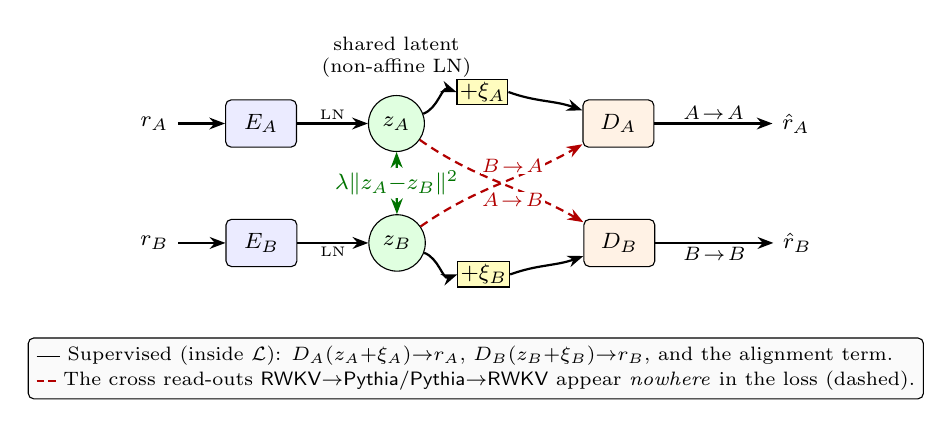
\begin{tikzpicture}[
  font=\footnotesize, >={Stealth[length=2mm]},
  box/.style={draw,rounded corners=2pt,minimum height=6mm,minimum width=9mm,align=center},
  enc/.style={box,fill=blue!8}, dec/.style={box,fill=orange!10},
  lat/.style={draw,circle,minimum size=7mm,fill=green!12,align=center},
  sup/.style={->,thick}, cross/.style={->,thick,densely dashed,red!70!black}]
\node (rA) {$r_A$};
\node[enc,right=6mm of rA] (EA) {$E_A$};
\node[lat,right=9mm of EA] (zA) {$z_A$};
\node[dec,right=20mm of zA] (DA) {$D_A$};
\node[right=15mm of DA] (rAo) {$\hat r_A$};
\node[below=11mm of rA] (rB) {$r_B$};
\node[enc,right=6mm of rB] (EB) {$E_B$};
\node[lat,right=9mm of EB] (zB) {$z_B$};
\node[dec,right=20mm of zB] (DB) {$D_B$};
\node[right=15mm of DB] (rBo) {$\hat r_B$};
\node[draw,fill=yellow!25,inner sep=1pt,right=4mm of zA,yshift=4mm] (nA) {$+\xi_A$};
\node[draw,fill=yellow!25,inner sep=1pt,right=4mm of zB,yshift=-4mm] (nB) {$+\xi_B$};
\draw[sup] (rA)--(EA); \draw[sup] (EA)--node[above,inner sep=1pt]{\tiny LN} (zA);
\draw[sup] (rB)--(EB); \draw[sup] (EB)--node[below,inner sep=1pt]{\tiny LN} (zB);
\draw[sup] (zA) to[out=20,in=160] (nA.west); \draw[sup] (nA.east) to[out=-20,in=160] (DA);
\draw[sup] (zB) to[out=-20,in=200] (nB.west); \draw[sup] (nB.east) to[out=20,in=200] (DB);
\draw[sup] (DA)--node[above,inner sep=1pt,font=\scriptsize]{$A\!\to\!A$}(rAo);
\draw[sup] (DB)--node[below,inner sep=1pt,font=\scriptsize]{$B\!\to\!B$}(rBo);
\draw[<->,thick,green!45!black] (zA)--node[fill=white,inner sep=1pt]{$\lambda\lVert z_A{-}z_B\rVert^2$} (zB);
\draw[cross] (zA) to[out=-35,in=150]
  node[pos=0.58,below=1pt,font=\scriptsize,fill=white,inner sep=0.5pt] {$A\!\to\!B$} (DB);
\draw[cross] (zB) to[out=35,in=210]
  node[pos=0.58,above=1pt,font=\scriptsize,fill=white,inner sep=0.5pt] {$B\!\to\!A$} (DA);
\node[align=center,above=1mm of zA,font=\scriptsize] {shared latent\\(non-affine LN)};
\node[draw,rounded corners=2pt,fill=gray!4,inner sep=3pt,font=\scriptsize,align=left,
      below=6mm of rB,anchor=north] at ($(rB)!0.5!(rBo)+(0,-6mm)$) {%
\textcolor{black}{\rule[0.4ex]{3mm}{0.7pt}}~Supervised (inside $\mathcal L$): $D_A(z_A{+}\xi_A){\to}r_A$, $D_B(z_B{+}\xi_B){\to}r_B$, and the alignment term.\\[1pt]
\textcolor{red!70!black}{\rule[0.4ex]{1mm}{0.7pt}\,\rule[0.4ex]{1mm}{0.7pt}}~The cross read-outs \RtoP{}/\PtoR{} appear \emph{nowhere} in the loss (dashed).};
\end{tikzpicture}
\caption{Shared-latent adapter. The residual of each frozen model is encoded into a \emph{single} latent $z$ (non-affine LayerNorm) and decoded back to its own
family (solid lines; these two reconstructions and the alignment term $\lambda\lVert z_A{-}z_B\rVert^2$ constitute the entire loss). Gaussian noise
$\xi_A,\xi_B\!\sim\!\mathcal N(0,\sigma^2)$ (independent) is added to $z$ \emph{only immediately before decoding} and does not enter the alignment term. The solid
$A\!\to\!A$ (\RWKVself{}) and $B\!\to\!B$ (\Pythiaself{}) are same-family reconstructions; the dashed
$A\!\to\!B$ (\RtoP{}) and $B\!\to\!A$ (\PtoR{}) are cross read-outs. The latter two are never fitted to a cross target
and become possible only once the alignment term makes $z_A{\approx}z_B$.}
\label{fig:adapter}
\end{figure*}

\paragraph{Adapter architecture.} $E_A,E_B,D_A,D_B$ share an identical form: a linear projection to the latent width, $b$
pre-norm residual blocks, and a linear projection to the output. The reported configuration is $z{=}d{=}4096$ (no compression), $b{=}1$, and internal width $h{=}4096$.
The second matrix of each residual block is \kw{zero-initialized}, so each block is initially the identity map and \emph{the adapter as a whole starts learning
from a linear map}. This, however, is a property of the initialization, not of the trained model: as measured in \S\ref{sec:linear}, after convergence
$13.4\%/12.0\%$ of the output variance of \RtoP{}/\PtoR{} is nonlinear, and the same nonlinear branch serves both cross read-outs.
Against the parents' combined $14.2$B parameters,
the adapter has $268.5$M ($1.9\%$). ``Lightweight'' refers not to absolute smallness but to the size relative to the parents and to the low depth.

\paragraph{Two design choices that matter.} The non-affine $\mathrm{LN}$ prevents the alignment term from being satisfied by shrinking $z$, and the noise $\xi$
is intended to suppress escape into a token-independent \emph{common mode} --- since a constant cannot evade the noise, $z$ is
forced to carry per-token information. We use a fixed $\sigma{=}0.4$ and do not sweep $\sigma$ in this paper.

\paragraph{Names of the four paths and the chimera.} In the equations we set $A$ to RWKV and $B$ to Tulu-Pythia, but
the main text and figures avoid the two-letter codes and state the prefix and suffix explicitly.
The four paths are \RWKVself{}, \RtoP{}, \Pythiaself{}, and \PtoR{}.
\RtoP{} and \PtoR{} are cross-family chimeras; \RWKVself{} and \Pythiaself{} are same-family reconstruction controls
that pass through the same boundary and adapter. The switch layer $L$ is the index (starting from $0$) of the last block the prefix parent executes,
not the number of layers executed --- since block $0$ is included, the prefix comprises $L{+}1$ blocks.
In \RtoP{}, we run the first $L{+}1$ blocks of $A$ (blocks $0$ through $L$)
and translate the residual into $B$ space exactly \emph{once}:
$h_B{=}\mathrm{unstd}_B(D_B(\mathrm{LN}(E_A(\mathrm{std}_A(h_A)))))$. We then run the remaining $31{-}L$
blocks of $B$ (from $L{+}1$ onward) and the language-model head. \PtoR{} is
evaluated separately with the same trained adapter,
inserting $h_A{=}\mathrm{unstd}_A(D_A(\mathrm{LN}(E_B(\mathrm{std}_B(h_B)))))$ into the input of RWKV block
$L{+}1$. In both cases the total is $32$ blocks, split as $L{+}1$ and $31{-}L$, with a single translation.
Correctness of the wiring is guaranteed by the boundary gate --- re-insertion of the suffix parent's own residual at the corresponding layer must recover the parent logits ---
and we confirmed $\mathrm{rel}{=}0$ at every boundary (see Appendix~\ref{sec:repro} for details of the check).

\paragraph{Evaluation metrics.} We measure the coefficient of determination $\Rsq$ on text not seen during training (pooling all tokens and all dimensions within a layer, with the SST centered per dimension) for both the cross-family mappings
($A\!\to\!B$, $B\!\to\!A$) and the same-family mappings ($A\!\to\!A$, $B\!\to\!B$). Latent alignment is measured with the \kw{centered}
correlation $\rho_{\mathrm{ctr}}$ (with the common mode removed), and we additionally report the fraction $f$ of the per-token varying component.
The two are linked to the alignment term through the relation $2f(1{-}\rho_{\mathrm{ctr}})$.
Each metric is computed per layer over all tokens (both the SST of $\Rsq$ and the common-mode removal for $\rho_{\mathrm{ctr}}$ and $f$ are done within each layer), and we report the simple mean over the $32$
layers. We never aggregate in one pool across layers --- differences among the per-layer means would inflate the apparent correlation and variance.
For the chimeras, we give English prompts verbatim and evaluate with generation samples produced by deterministic argmax at temperature $0$ (at most $40$ new tokens,
early stopping only on EOS output), multiple-choice accuracy, and next-token cross-entropy.

\section{A Learnable Shared Representation Exists Between Corresponding Layers (Under Favorable Conditions)}\label{sec:space}
For the pair of $7$B instruction-following models RWKV-Raven-7B (pure RNN) $\leftrightarrow$ Tulu-Pythia-6.9b (Transformer), both with $32$ blocks,
$d{=}4096$, and a shared GPT-NeoX tokenizer, aligning on instruction-formatted text (Alpaca) lets an adapter consisting of 1 residual block
reach a centered latent correlation of $\rho_{\mathrm{ctr}}\!=\!0.901$ on unseen text. Because the raw correlation ($0.97$) can be inflated by the
common mode, we do not take it as evidence by itself. We take the centered correlation of $0.901$, together with the fact that each decoder can reconstruct residuals of its own family
($A\!\to\!A\ 0.70$, $B\!\to\!B\ 0.71$), as the grounds for a shared representation. Moreover, even the best \emph{linear} map fitted directly
to each cross read-out task reaches $A\!\to\!B\ 0.487$ and $B\!\to\!A\ 0.535$ (\S\ref{sec:linear}). Hence a large part of the observed
predictability cannot be explained by the expressive power of the deep nonlinear map alone.
However, \kw{same-index layer pairs are not intrinsically special}: comparing raw residuals, without any adapter, across all $32{\times}32$ layer pairs (Fig.~\ref{fig:cka}),
linear CKA is weak throughout (diagonal mean $0.05$ vs. off-diagonal mean $0.03$), and layer $j$ of $A$ is most similar to layer $j$ of $B$ in only
$2$ of $32$ rows (the most similar layer is layer $0$ in $14$ rows and the final layer in $12$ rows). Nor are same-index layers special in direct linear regressability:
fitting per-layer linear maps to the same full set of layer pairs yields fit $R^2$ with a diagonal mean of $0.87$ vs. an off-diagonal mean of $0.84$,
and the same-numbered layer is best in only $3$ of $32$ rows. Hence $\rho_{\mathrm{ctr}}\!=\!0.901$ is an alignment \emph{learned and
recovered on the chosen same-index layer pairs}, not a correspondence intrinsic to matching layer indices --- it should be read as the choice of
same-index layers laid on top of a regressability that exists for almost any layer pair.

\begin{figure}[!htbp]\centering
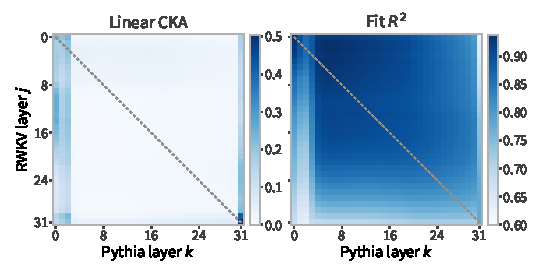
\includegraphics[width=\columnwidth]{fig_layer_cka_en}
\caption{All $32{\times}32$ layer correspondences of raw residuals (generated from the canonical table \texttt{paper\_layer\_correspondence.csv}).
Left: linear CKA is weak throughout, and high values concentrate in the row and column of layer $0$ and the corner of the final layer --- the diagonal (dashed) is not special.
Right: the fit $R^2$ of per-layer linear maps fitted to the same pairs is high for nearly all pairs, at $0.62$--$0.94$.
The color scales of the two panels differ.}
\label{fig:cka}
\end{figure}We can confirm that the alignment is \emph{learnable},
but in this sense as well its scope is limited (\S\ref{sec:discussion}).

All numbers below come from a single training run of the same configuration. The latent width is $z{=}d{=}4096$ (no compression), all $32$ blocks
are paired, the adapter has $268.5$M parameters, $\sigma{=}0.4$, and the learning rate was decayed from $10^{-3}$ by a plateau schedule down to a floor of $10^{-5}$.
The training signal consists of residuals taken from $2{,}075$ windows of the Alpaca training split (each $112$ tokens; $\approx\!232$k independent token positions),
forming $7.44$M pairs across the $32$ layers, and this pair set was iterated over about $228$ times. Reported values are from the checkpoint at the
deepest point ($415{,}000$ iterations) where held-out $A\!\to\!B$ is best (training runs and convergence records are in Appendix~\ref{sec:repro}). The \PtoR{} cross-family map attains $B\!\to\!A\ 0.590$, slightly above
$A\!\to\!B\ 0.559$ (residuals on the RNN side are easier to recover from the Transformer latent). Both fall below same-family reconstruction
($A\!\to\!A\ 0.695$, $B\!\to\!B\ 0.711$), corroborating that cross-family transfer is bottlenecked by decoding rather than by alignment.
That these alignments and read-outs are a true per-token correspondence rather than distributional overlap was verified with a negative control: keeping the row order of $A$ fixed
while re-pairing the residual rows of $B$ under a single random permutation collapses $\rho_{\mathrm{ctr}}$ from $0.901\!\to\!0.000$,
$A\!\to\!B$ from $0.561\!\to\!-0.592$, and $B\!\to\!A$ from $0.592\!\to\!-0.609$
(the same-family maps $A\!\to\!A$, $B\!\to\!B$ are unchanged by construction). That is, neither direction of read-out is obtainable without the correct token correspondence.

\paragraph{The common mode is not a trivial issue.}Introducing the fraction of the latent that varies per token,
$f=\lVert z-\overline{z}\rVert^2/\lVert z\rVert^2$, quantifies this pitfall. Under layer normalization without
elementwise gains, the raw correlation decomposes as
$\rho_{\mathrm{raw}}=(1-f)+f\,\rho_{\mathrm{ctr}}$, i.e., $\text{align}=2f(1-\rho_{\mathrm{ctr}})$.
The $f$ reported here is the mean of the varying fractions of $A$ and $B$ respectively, and this form holds as an equality when the two are equal
and their common modes are parallel. As measured, at evaluation points after training has progressed this relation holds to a precision of about
$3\!\times\!10^{-4}$. It does not hold early in training, however: at iteration $0$ the residual reaches $6.6\!\times\!10^{-2}$. What the equality tells us is that the raw correlation is a \emph{mixture}
--- of which a fraction $1-f$ is given for free as a constant term carrying no information. Since $f$ at the deepest point is $0.350$,
\kw{$65\%$ of the latent's energy is a token-independent constant}, and the raw correlation is dominated by that constant. Indeed, whereas the centered
$\rho_{\mathrm{ctr}}$ is $0.901$, the raw correlation reads $0.965$, and the equality reproduces this exactly as
$(1{-}0.350)+0.350\times0.901=0.965$. The interpretive limits of $f$ (a large $f$ does not necessarily carry
information) and a concrete example of training dynamics in which the raw correlation fails to capture improvement are given in Appendix~\ref{sec:common-mode}.

\section{Both Cross Read-Outs Are Constrained by Same-Family Reconstruction}\label{sec:ladder}
Fig.~\ref{fig:ladder} shows the five measured diagnostic values.
\[
 \begin{array}{ll}
 \multicolumn{2}{l}{\rho_{\mathrm{ctr}}=0.901,}\\
 \Rsq(B\!\to\!B)=0.711, & \Rsq(A\!\to\!B)=0.559,\\
 \Rsq(A\!\to\!A)=0.695, & \Rsq(B\!\to\!A)=0.590 .
 \end{array}
\]
$\rho_{\mathrm{ctr}}$ is a correlation coefficient, whereas the latter four are coefficients of determination; their magnitudes cannot be compared as if on the same scale.
The conclusions of this section rest on the facts that, among the $\Rsq$ values, $A\!\to\!B\le B\!\to\!B$ and $B\!\to\!A\le A\!\to\!A$ hold in all $32$ layers, and that in the autoencoder contrast of \S\ref{sec:goal} the decode-only loss also manifests in downstream performance.

\begin{figure*}[!t]\centering
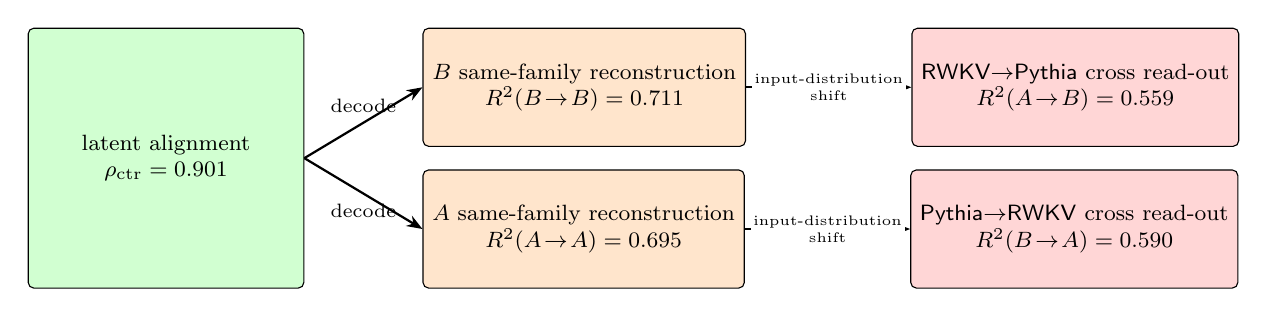
\begin{tikzpicture}[
  font=\footnotesize, >={Stealth[length=2mm]},
  diag/.style={draw,rounded corners=2pt,minimum width=35mm,minimum height=15mm,align=center}]
  \node[diag,fill=green!18,minimum height=33mm] (align) {latent alignment\\$\rho_{\mathrm{ctr}}=0.901$};
  \node[diag,fill=orange!20,right=15mm of align,yshift=9mm] (selfb)
    {$B$ same-family reconstruction\\$\Rsq(B\!\to\!B)=0.711$};
  \node[diag,fill=red!16,right=21mm of selfb] (crossab)
    {\RtoP{} cross read-out\\$\Rsq(A\!\to\!B)=0.559$};
  \node[diag,fill=orange!20,right=15mm of align,yshift=-9mm] (selfa)
    {$A$ same-family reconstruction\\$\Rsq(A\!\to\!A)=0.695$};
  \node[diag,fill=red!16,right=21mm of selfa] (crossba)
    {\PtoR{} cross read-out\\$\Rsq(B\!\to\!A)=0.590$};
  \draw[->,thick] (align.east)--node[above,font=\scriptsize]{decode} (selfb.west);
  \draw[->,thick] (align.east)--node[below,font=\scriptsize]{decode} (selfa.west);
  \draw[->,thick] (selfb)--node[midway,fill=white,inner sep=1pt,font=\tiny,align=center]
    {input-distribution\\shift} (crossab);
  \draw[->,thick] (selfa)--node[midway,fill=white,inner sep=1pt,font=\tiny,align=center]
    {input-distribution\\shift} (crossba);
\end{tikzpicture}
\caption{Diagnostic values from the shared latent to the read-outs in both directions. High centered correlation coexists with imperfect self-reconstruction, and the \RtoP{}/\PtoR{} cross read-outs fall below, in all layers, the \Pythiaself{}/\RWKVself{} self-reconstructions that use the same respective decoders.
Because a correlation coefficient and a coefficient of determination are different scales, we do not interpret the numeric gap between the scales itself as an amount of loss.}
\label{fig:ladder}
\end{figure*}
High latent correlation does not automatically guarantee high reconstruction accuracy. \RtoP{} can be compared with \Pythiaself{}, which passes through the same decoder $D_B$, and
\PtoR{} with \RWKVself{}, which passes through the same decoder $D_A$; the only difference is whether the input is a same-family or a cross-family latent.
Both inequalities are empirical observations rather than theorems, but in either direction a substantial error is already present at the self-reconstruction stage,
and improving only the cross-family step leaves that error in place.

\paragraph{Compression cannot explain it, but the cause of the ceiling remains unresolved.}One could object that $B\!\to\!B$ is low simply because the latent compresses
information. This can be checked not by argument but by removing the compression itself. At $z{=}d{=}4096$
the composite map $D\!\circ\!E$ can represent the identity map, and no rank constraint exists. Even so, $B\!\to\!B$ remains at
$0.711$. Is it, then, a ceiling set by the noise $\sigma$? A simple scalar approximation cannot explain $0.711$, and what is rate-limiting
cannot be determined until $\sigma$ is swept, so we leave this \emph{unresolved} in this paper. Note that $\sigma$ plays another role---suppressing collapse into the common mode---which the trajectory of $f$
supports, and that point is unchanged: removing compression alone does not resolve the problem; even with the wide latent, $98\%$ of the latent energy
collapses to a constant early in training, and recovery is slow until the final phase of training (the trajectory of $f$ is given in Appendix~\ref{sec:common-mode}). This is a degeneracy that persists even when a wide latent is
used, and it is also the reason the common-mode correction is not a trivial issue.

\section{The Adapter Is Nonlinear on Both Cross Paths}\label{sec:linear}
The adapter is a single zero-initialized residual block sandwiched between two linear maps, so training begins from a purely linear map. But that is a property at iteration
$0$, not after $415{,}000$ iterations. We measured how linear the adapter at the deepest point actually is,
for both \RtoP{} and \PtoR{}, on the same $5$ representative layers and the same fit and held-out rows.

\emph{How much of the adapter is linear.} The best affine map mimicking the adapter's own output explains
$86.6\%$ of the output variance for \RtoP{} and $88.0\%$ for \PtoR{}. Hence \kw{the remaining $13.4\%$/$12.0\%$
cannot be expressed by any affine map}. The fact that the second matrix is zero-initialized speaks only to initialization;
the trained map is clearly nonlinear on both paths.

\emph{How far a linear map alone can reach.} The comparison is not an approximation of the adapter: it is a control obtained by \emph{directly} fitting,
per layer and separately for each path, the best affine map from the standardized input residuals to the standardized output residuals via ridge least squares
(see Appendix~\ref{sec:repro} for setup details). Evaluated on the held-out rows of the $5$ representative layers $\{4,10,16,22,28\}$,
the best direct affine map reaches $0.487$ for \RtoP{} and $0.535$ for \PtoR{}. The corresponding adapter, on the same rows, achieves $0.558$ for \RtoP{} and $0.576$ for \PtoR{},
so the nonlinear map's increment is $+0.071$/$+0.041$. Because even a low-capacity affine map achieves substantial
cross-family prediction on both paths, \emph{the shared-representation claim is underwritten by this linear reachability}.

\emph{The separately fitted affine control.} In Table~\ref{tab:bench}, replacing the \RtoP{} adapter with the direct affine map
collapses accuracy by $8$--$23$ points. For \PtoR{}, by contrast, the gap is small, and on SciQ @8 the affine control is $3.4$ points higher.
This matters as a path difference, but because the two maps differ in training objective, data, and regularization, we do not treat it as a causal effect of nonlinearity.

\emph{A confound-controlled intervention: disabling the MLP branch of the same adapter.} We therefore scale only the
residual block of \kw{the same trained adapter} (its sole learned nonlinearity, $\mathrm{fc}_2(\mathrm{GELU}(\mathrm{fc}_1(\cdot)))$) by a coefficient $\alpha$
($\alpha{=}1$ intact; $\alpha{=}0$ is \emph{the identical map with the branch removed}).
Sweeping representation $R^2$ over $\alpha=0,.25,.5,.75,1$ yields
$-0.41,-0.75,0.35,0.52,0.56$ for \RtoP{} and $-0.30,-0.66,0.36,0.53,0.58$ for \PtoR{}.
On both paths, removing the branch collapses performance all the way to negative $R^2$, and moreover the sweep is non-monotonic. The two linear layers were trained
in coordination with the residual block, and \kw{in this trained adapter, the nonlinear branch cannot be removed from the read-out of \PtoR{} any more than from \RtoP{}}.
This is a property of the trained map and does not mean the task is in principle unsolvable by a linear map (we did not compare against a
linear adapter trained with the same objective). For multiple choice as well, we evaluate the same $\alpha=0/1$ pair
on identical questions in paired fashion.

\begin{table}[!htbp]\centering\scriptsize
\caption{Length-normalized accuracy (\%) when the nonlinear branch of the same adapter is disabled.
Each cell shows $\alpha:1\!\to\!0$ (full trained map $\to$ the same map with only the branch removed).
ARC-Easy $2376$, SciQ $1000$, chance $25\%$.}\label{tab:mlp-intervention}
\setlength{\tabcolsep}{4.2pt}
\resizebox{\columnwidth}{!}{%
\begin{tabular}{rcccc}\toprule
& \multicolumn{2}{c}{ARC-Easy} & \multicolumn{2}{c}{SciQ}\\
\cmidrule(lr){2-3}\cmidrule(lr){4-5}
$L$ & \RtoP{} & \PtoR{} & \RtoP{} & \PtoR{}\\\midrule
4  & $59.6\!\to\!31.9$ & $62.2\!\to\!31.8$ & $70.9\!\to\!31.3$ & $69.2\!\to\!32.6$\\
8  & $59.0\!\to\!29.9$ & $57.3\!\to\!35.5$ & $67.7\!\to\!31.4$ & $64.6\!\to\!37.0$\\
16 & $48.6\!\to\!28.5$ & $57.5\!\to\!43.7$ & $54.5\!\to\!31.7$ & $68.0\!\to\!47.3$\\
24 & $47.0\!\to\!34.8$ & $59.6\!\to\!48.4$ & $51.1\!\to\!40.0$ & $69.9\!\to\!49.1$\\\bottomrule
\end{tabular}}
\end{table}

The branch effect in Table~\ref{tab:mlp-intervention} is $+11.1$--$+39.6$ points for \RtoP{} and
$+11.2$--$+36.6$ points for \PtoR{}, and an exact McNemar test on identical questions gives
$p<2{\times}10^{-9}$ in all $16$ comparisons. Hence the necessity of the nonlinear branch is not inferred from one path alone:
it is confirmed directly in both the \RtoP{} and \PtoR{} representations and in downstream accuracy.

\section{Syntactically Plausible Generation, Degraded Factuality}\label{sec:chimera}
Here we actually compose both cross-family paths at $7$B. At switch layer $L$, we run the prefix parent from block $0$ through $L$
(a total of $L{+}1$ blocks), translate its residual \emph{once} into the other space via the boundary formula of \S\ref{sec:method},
and then run the suffix parent's blocks from $L{+}1$ onward together with its language-model head---not a per-block round trip.
Thus \RtoPL{16} uses $17$ RWKV blocks and $15$ Pythia blocks, and \PtoRL{16} the reverse; neither is an exact half.

\begin{figure*}[!t]\centering
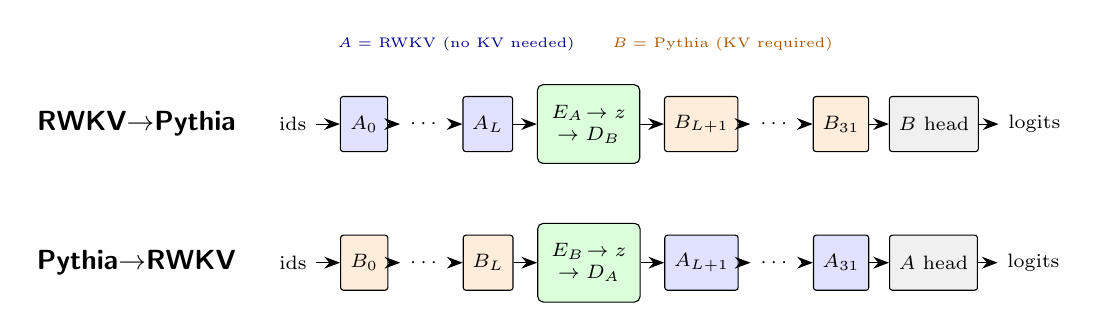
\begin{tikzpicture}[
  font=\scriptsize, >={Stealth[length=2mm]},
  a/.style={draw,rounded corners=1pt,minimum height=7mm,minimum width=6mm,fill=blue!12},
  b/.style={draw,rounded corners=1pt,minimum height=7mm,minimum width=6mm,fill=orange!14},
  hd/.style={draw,rounded corners=1pt,minimum height=7mm,minimum width=8mm,fill=gray!12},
  tr/.style={draw,rounded corners=2pt,minimum height=10mm,minimum width=13mm,fill=green!14,align=center}]
% \RtoP{} row
\node[font=\bfseries] (labAB) {\RtoP{}};
\node[right=3mm of labAB] (idsAB) {ids};
\node[a,right=3mm of idsAB] (a0) {$A_0$};
\node[right=1.5mm of a0] (ad) {$\cdots$};
\node[a,right=1.5mm of ad] (aL) {$A_L$};
\node[tr,right=3mm of aL] (tab) {$E_A\!\to z$\\$\to D_B$};
\node[b,right=3mm of tab] (bN) {$B_{L+1}$};
\node[right=1.5mm of bN] (bd) {$\cdots$};
\node[b,right=1.5mm of bd] (b31) {$B_{31}$};
\node[hd,right=2.5mm of b31] (hb) {$B$ head};
\node[right=2.5mm of hb] (outAB) {logits};
\draw[->] (idsAB)--(a0);
\foreach \x/\y in {a0/ad,ad/aL,aL/tab,tab/bN,bN/bd,bd/b31,b31/hb,hb/outAB} \draw[->] (\x)--(\y);
% \PtoR{} row, aligned by role with \RtoP{}
\node[font=\bfseries,below=12mm of labAB] (labBA) {\PtoR{}};
\node[right=3mm of labBA] (idsBA) {ids};
\node[b,right=3mm of idsBA] (bb0) {$B_0$};
\node[right=1.5mm of bb0] (bbd) {$\cdots$};
\node[b,right=1.5mm of bbd] (bbL) {$B_L$};
\node[tr,right=3mm of bbL] (tba) {$E_B\!\to z$\\$\to D_A$};
\node[a,right=3mm of tba] (aaN) {$A_{L+1}$};
\node[right=1.5mm of aaN] (aad) {$\cdots$};
\node[a,right=1.5mm of aad] (aa31) {$A_{31}$};
\node[hd,right=2.5mm of aa31] (ha) {$A$ head};
\node[right=2.5mm of ha] (outBA) {logits};
\draw[->] (idsBA)--(bb0);
\foreach \x/\y in {bb0/bbd,bbd/bbL,bbL/tba,tba/aaN,aaN/aad,aad/aa31,aa31/ha,ha/outBA} \draw[->] (\x)--(\y);
\node[font=\tiny,above=3mm of tab,align=center] {
  \textcolor{blue!55!black}{$A=$ RWKV (no KV needed)}\qquad
  \textcolor{orange!65!black}{$B=$ Pythia (KV required)}
};
\end{tikzpicture}
\caption{Symmetric construction of the \RtoP{}/\PtoR{} chimeras. The parent on the left of the figure runs up to block $L$; its residual is translated once and
passed to the right parent's blocks from $L{+}1$ onward and its head. Blue is RWKV-Raven, orange is Tulu-Pythia.
The number of Transformer layers is therefore $31{-}L$ for \RtoP{} and $L{+}1$ for \PtoR{}.}
\label{fig:chimera}
\end{figure*}

We insert the same deepest-point adapter at $L{=}4$ for both \RtoP{} and \PtoR{}, and greedily decode the same four English prompts
at temperature $0$ with at most $40$ new tokens. $L{=}4$ is the boundary at which the two-task average is largest among the four boundaries in each cross-family direction,
and it is the common boundary at which both directions enter the non-dominated set on the SciQ KV--accuracy plane (Fig.~\ref{fig:tradeoff}).
This is, however, a representative-point selection made after seeing the same reported tasks, not an independent selection criterion for generation.
This comparison is not an exhaustive generation benchmark, but at least it does not infer one direction's generation from the other's cross read-out;
we observe both end-to-end wirings under identical conditions.

\begin{table*}[!t]\centering\footnotesize
\setlength{\tabcolsep}{4pt}
\caption{Regeneration results of the deepest-point adapter via \RtoP{}/\PtoR{} (both $L{=}4$), together with the outputs of the two parents,
pure Pythia and pure RWKV, on the same prompts. The English originals were fed verbatim, using temperature $0$ argmax, at most $40$ new tokens, and early stopping on EOS only.
Each chimera is placed next to its suffix parent. Long repetitions are summarized; the verbatim outputs are recorded in
\texttt{paper\_cross\_family\_generation\_samples.csv}.
This is a qualitative comparison limited to four prompts, not a quantitative evaluation of generation quality.}\label{tab:generation}
\begin{tabular}{|p{0.145\linewidth}|p{0.18\linewidth}|p{0.19\linewidth}|p{0.16\linewidth}|p{0.19\linewidth}|}\hline
Prompt (verbatim) & pure Pythia &
\RtoP{}\par{\scriptsize cross read-out $R^2{=}0.559$} &
pure RWKV &
\PtoR{}\par{\scriptsize cross read-out $R^2{=}0.590$}\\\hline
{\ttfamily \#\#\# Instruction:\par
What is the capital of France?\par\smallskip
\#\#\# Response:} &
``The capital of France is Paris.'' & \textbf{``The capital of France is Paris.''} \checkmark &
``Paris.'' & \textbf{``Paris.''} \checkmark\\\hline
{\ttfamily The three primary colors are} &
``red, yellow, and blue. These colors are often used in combination to create a wide variety of colors.'' & \textbf{``red, yellow, and blue.''} \checkmark &
Correct with ``red, blue, and yellow.'', then drifts into a Q\&A asking for the opposite color of red (green) &
Correct with ``red, blue, and yellow.'', then drifts into a Bob/Alice dialogue about green\\\hline
{\ttfamily Question: Water is made of hydrogen and\par Answer:} &
``Hydrogen is made of hydrogen and oxygen.'' &
``Hydrogen.'' \textbf{(incorrect)} &
``hydrogen.'' \textbf{(incorrect)} & ``hydrogen.'' \textbf{(incorrect)}\\\hline
{\ttfamily \#\#\# Instruction:\par
Explain what a black hole is in one sentence.\par\smallskip
\#\#\# Response:} &
``A black hole is a region of spacetime where gravity is so strong that nothing, not even light, can escape its pull.'' &
``A black hole is a region in space where gravity is so strong that nothing, not even light, can escape its pull.'' \checkmark &
``A black hole is a region of space where the gravitational pull is so strong that nothing, not even light, can escape.'' &
``A black hole is a type of celestial object that is formed when a star collapses and collapses into a black hole.''
\emph{(circular)}\\\hline
\end{tabular}
\end{table*}

Two points can be observed from these examples. First, \kw{both \RtoP{} and \PtoR{} can generate syntactically plausible output}. Both answer the capital of France correctly,
and both start the primary colors correctly. \RtoP{} also answers the black-hole prompt correctly in one sentence, so this is not behavior
inferred from the representation metric of only one direction. Second, \kw{fluency can be preserved while content or instruction format is lost}. Both directions complete the water prompt
incorrectly with ``hydrogen'', and \PtoR{} drifts into a dialogue format after correctly answering the primary colors and explains the black hole circularly.
Thus even cross read-outs of $0.559/0.590$ are not sufficient for factuality. A more faithful chimera requires improving both cross read-outs
and same-family reconstruction.

\section{Function and Inference-Memory Comparison Against the Parents}\label{sec:goal}
Assessing the practical value of NinaXander requires a functional comparison against the frozen parents, not internal-representation metrics alone.
Here we measure (i) how much performance can be retained relative to the strong parent, (ii) whether the weak parent or a
Transformer with the same KV capacity is surpassed, and (iii) how much memory is saved in exchange.

This comparison is run in a multiple-choice format that computes the log-likelihood of each option and selects the maximum. Because no generation, string matching, or subjective judgment
is involved, the result is uniquely determined. We used the \kw{full evaluation sets} (ARC-Easy test $2376$, SciQ test $1000$), the $z{=}4096$ adapters at the deepest point
($415{,}000$ iterations), and four switch positions. Between-configuration comparisons on the same question set are paired data, so
differences are assessed with \kw{paired tests} (McNemar's exact test and paired bootstrap) rather than independent per-cell binomial SEs. Because the options differ in
length and sum vs.\ length-normalized scoring can disagree in ranking, both are stored in the structured data, and the main text uses length-normalized scoring for reporting and testing.
Moreover, SciQ is evaluated in a closed-book format (Question/Answer only) that does not supply the accompanying support passages, so the SciQ values in this paper
are not directly comparable to published values under the standard protocol that provides support.

\begin{table}[!htbp]\centering\scriptsize
\caption{Length-normalized multiple-choice accuracy (\%, ARC-Easy $2376$, SciQ $1000$, chance $25$) for the trained \RtoP{}/\PtoR{} adapters
and the best affine controls fitted separately to each path's input and output residuals.
Each value uses the same questions, the same switch layer, and the same suffix execution.}\label{tab:bench}
\setlength{\tabcolsep}{2.8pt}
\resizebox{\columnwidth}{!}{%
\begin{tabular}{rcccccccc}\toprule
& \multicolumn{4}{c}{ARC-Easy} & \multicolumn{4}{c}{SciQ}\\
\cmidrule(lr){2-5}\cmidrule(lr){6-9}
& \multicolumn{2}{c}{\RtoP{}} & \multicolumn{2}{c}{\PtoR{}}
& \multicolumn{2}{c}{\RtoP{}} & \multicolumn{2}{c}{\PtoR{}}\\
$L$ & adapter & affine & adapter & affine
& adapter & affine & adapter & affine\\\midrule
4  & 59.6 & 41.9 & 62.2 & 60.2 & 70.9 & 47.5 & 69.2 & 69.6\\
8  & 59.0 & 43.1 & 57.3 & 56.0 & 67.7 & 49.1 & 64.6 & 68.0\\
16 & 48.6 & 34.8 & 57.5 & 57.5 & 54.5 & 35.9 & 68.0 & 69.6\\
24 & 47.0 & 39.4 & 59.6 & 59.2 & 51.1 & 42.7 & 69.9 & 68.2\\\bottomrule
\end{tabular}}
\end{table}

\begin{table}[!htbp]\centering\scriptsize
\caption{Length-normalized accuracy (\%) of the four paths.
\RWKVself{}/\Pythiaself{} are same-family reconstruction controls; \RtoP{}/\PtoR{} are cross-family chimeras.
Differences between the two cross paths on the same questions and switch layer were paired and tested.}
\label{tab:direction}
\setlength{\tabcolsep}{3.2pt}
\resizebox{\columnwidth}{!}{%
\begin{tabular}{rcccccccc}\toprule
& \multicolumn{2}{c}{\RWKVself{}} & \multicolumn{2}{c}{\RtoP{}}
& \multicolumn{2}{c}{\Pythiaself{}} & \multicolumn{2}{c}{\PtoR{}}\\
$L$ & ARC & SciQ & ARC & SciQ & ARC & SciQ & ARC & SciQ\\\midrule
4  & 62.8 & 68.5 & 59.6 & 70.9 & 62.2 & \textbf{74.8} & \textbf{62.2} & 69.2\\
8  & 59.8 & 66.7 & 59.0 & 67.7 & 62.7 & \textbf{74.8} & 57.3 & 64.6\\
16 & 54.8 & 59.8 & 48.6 & 54.5 & 57.4 & \textbf{71.1} & \textbf{57.5} & 68.0\\
24 & 52.2 & 57.9 & 47.0 & 51.1 & 59.4 & \textbf{70.1} & \textbf{59.6} & 69.9\\\bottomrule
\end{tabular}}
\end{table}

Six observations follow from the joint comparison of the four paths. \emph{(a)} \kw{Even with half of the $7$B being foreign, both \RtoP{} and \PtoR{} can actually
answer the questions}. All cross configurations far exceed chance, reaching \RtoP{} $70.9\%$ and \PtoR{} $69.9\%$ on SciQ.
\emph{(b)} \kw{The depth effect is path-dependent}. \RtoP{} decreases monotonically over $L=4\to24$, SciQ
$70.9\to67.7\to54.5\to51.1$ and ARC-Easy $59.6\to59.0\to48.6\to47.0$, whereas
\PtoR{} is non-monotonic, SciQ $69.2\to64.6\to68.0\to69.9$ and ARC-Easy $62.2\to57.3\to57.5\to59.6$.
Local read-out at the same four layers is \RtoP{} $0.570/0.555/0.575/0.567$ and \PtoR{} $0.552/0.517/0.604/0.608$,
so the end-to-end ranking is not determined by the layer index or a single local $R^2$ alone.
\emph{(c)} \kw{The stronger parent is not surpassed on either path}. All $8$ cross configurations fall below Tulu-Pythia on both tasks,
and the differences are significant under McNemar tests on the same questions in every case.
\emph{(d)} \kw{The difference against RWKV is likewise path- and task-dependent}. \RtoPL{4} exceeds RWKV by $+3.9$ points on SciQ
($p{=}0.018$) but is $-2.2$ points on ARC-Easy ($p{=}0.042$). Under sum scoring, however, this advantage disappears
(\RtoPL{4} is $-2.7$ points on SciQ; \PtoRL{4} is $-4.6$ points on ARC / $-5.7$ points on SciQ) --- the verdict against the weaker parent depends on
the choice of length normalization. \PtoR{} does not significantly exceed RWKV at any boundary,
and \PtoRL{4} is statistically equivalent at ARC $+0.4$ points ($p{=}0.66$) and SciQ $+2.2$ points ($p{=}0.14$).
\emph{(e)} \kw{The difference against the separately fitted affine controls is also path-dependent}. On \RtoP{} the adapter is $8$--$23$ points higher in every cell,
whereas on \PtoR{} the differences are small, and at SciQ @8 the affine is $3.4$ points higher. This comparison is descriptive because the mappings themselves differ;
the causal comparison that manipulates the nonlinear branch of the same adapter is carried out for both paths via the $\alpha$ intervention in \S\ref{sec:linear}.
\emph{(f)} \kw{The gap to the same-family controls is not translation error alone}. With the B suffix, accuracy decreases in the order pure Pythia, \Pythiaself{}, \RtoP{},
with \Pythiaself{}--\RtoP{} gaps of SciQ $4$--$19$ points and ARC $3$--$12$ points. With the A suffix, by contrast, \PtoR{} conversely exceeds \RWKVself{} at deep boundaries,
and the differences at $L=16/24$ are ARC $+2.7/+7.4$ points and SciQ $+8.2/+12.0$ points.
The same-family controls therefore isolate the decode stage, but the gap to the cross paths contains both the prefix parent's capability and translation mismatch,
and does not constitute a universal ``translation cost.''

\paragraph{Depth dependence differs between \RtoP{} and \PtoR{}.}As Table~\ref{tab:direction} shows, at $L{=}16,24$ \PtoR{} exceeds the same-layer \RtoP{} by
$+8.9/+12.6$ points on ARC and $+13.5/+18.8$ points on SciQ (McNemar tests on the same questions, all
$p<3{\times}10^{-15}$). At $L{=}4$, on the other hand, the difference is $+2.6$ points on ARC ($p{=}0.015$) but $-1.7$ points on SciQ
($p{=}0.28$), so at shallow boundaries the path difference is not uniform. Hence the monotonic depth effect seen for \RtoP{} cannot be generalized as
``the difficulty of joining layers with the same index.'' Every \PtoR{} configuration falls significantly below Pythia. Nor is there any \PtoR{} configuration that significantly exceeds RWKV;
\PtoRL{4} is equivalent at ARC $62.2$ vs.\ $61.8$ ($p{=}0.66$) and SciQ $69.2$ vs.\ $67.0$ ($p{=}0.14$).

The best affine mapping for \PtoR{} is a control fitted separately from the adapter at each switch layer. At ARC @4 the adapter is $+2.0$ points higher
($p{=}0.005$), but most of the other cells show no difference, and at SciQ @8 the affine is conversely $+3.4$ points higher ($p{=}0.003$).
Separately from this between-mapping comparison, the intervention that sets the nonlinear branch of the same adapter to $\alpha=0$ is executed for \RtoP{}/\PtoR{} at the same four layers and the same questions,
and the causal contribution of the nonlinear branch is assessed from those paired results. The comparison with the $A\!\to\!A$ autoencoder likewise
replaces the RWKV prefix simultaneously with a Pythia prefix and cross translation, and thus does not isolate translation error alone.

\paragraph{The released defaults are ``best measured'' selections, not external validation.}Averaging the accuracies of the two tasks, \PtoRL{4} is
$65.70\%$ and \RtoPL{4} is $65.25\%$, a difference of only $0.45$ points. The full release splits by path explicitly:
\nolinkurl{ninaxander-tulu69-to-raven7b-best} sets \PtoRL{4}, and
\nolinkurl{ninaxander-raven7b-to-tulu69-best} sets \RtoPL{4}, as the default within each path.
The runtime refuses switching to the path opposite to the package name, while retaining the $L{=}8,16,24$ plans for boundary comparison.
Both are \emph{post-hoc} rankings selected from each path's four boundaries on the same two reported test sets, and there is no independent
deployment-selection split. They are therefore not used as grounds for claiming improvement on unseen execution paths in general or superior generalization performance.

\paragraph{The memory effect of composition: the KV cache disappears together with the Transformer layers.}Performance and inference memory must be evaluated jointly,
because the two families do not have the same inference-time cost. Transformer layers cache key/value per token,
whereas an RNN layer carries only a recurrent state that is \kw{$O(1)$ in sequence length}. \RtoP{} retains only $31{-}L$ Transformer layers,
and \PtoR{} only $L{+}1$. The Tulu-Pythia cache was \emph{measured}, not assumed:
$16.0$ KiB/token per layer, $512$ KiB/token over $32$ layers (in exact agreement with $2Ld\cdot2$\,bytes).

\begin{table*}[!t]\centering\footnotesize
\caption{Accuracy and inference memory for both \RtoP{}/\PtoR{} paths. KV is measured; the RWKV recurrent state is constant in context length.}\label{tab:kv}
\begin{tabular}{lccccc}\toprule
Configuration & Transformer layers & KV / token & KV @ $4$k context & Reduction & ARC / SciQ\\\midrule
pure Tulu-Pythia & 32 & $512$ KiB & $2.00$ GiB & --- & 65.3 / 81.0\\
\RtoPL{4}  & 27 & $432$ KiB & $1.69$ GiB & $15.6\%$ & 59.6 / 70.9\\
\RtoPL{8}  & 23 & $368$ KiB & $1.44$ GiB & $28.1\%$ & 59.0 / 67.7\\
\RtoPL{16} & 15 & $240$ KiB & $0.94$ GiB & $53.1\%$ & 48.6 / 54.5\\
\RtoPL{24} &  7 & $112$ KiB & $0.44$ GiB & $78.1\%$ & 47.0 / 51.1\\
\PtoRL{24} & 25 & $400$ KiB & $1.56$ GiB & $21.9\%$ & 59.6 / 69.9\\
\PtoRL{16} & 17 & $272$ KiB & $1.06$ GiB & $46.9\%$ & 57.5 / 68.0\\
\PtoRL{8}  &  9 & $144$ KiB & $0.56$ GiB & $71.9\%$ & 57.3 / 64.6\\
\textbf{\PtoRL{4}} & \textbf{5} & \textbf{$80$ KiB} & \textbf{$0.31$ GiB} &
\textbf{$84.4\%$} & \textbf{62.2 / 69.2}\\
pure RWKV-Raven & 0 & $0$ & $0$ & $100\%$ & 61.8 / 67.0\\\bottomrule
\end{tabular}
\end{table*}

Including \RtoP{}/\PtoR{}, \PtoRL{4} reduces the Transformer layers from $27\to5$ relative to \RtoPL{4} while nearly preserving the two-task average,
$65.25\%\to65.70\%$. The recurrent state of the replacing RWKV is $40$ KiB per layer (a computed value from $5$ state vectors ${\times}\,4096$ dimensions ${\times}$ fp16) and is by construction independent of context length.
However, pure RWKV has zero KV and the ranking is task-dependent, so Fig.~\ref{fig:tradeoff} is presented as a
memory--accuracy frontier restricted to SciQ.

\begin{figure}[!htbp]\centering
\resizebox{\columnwidth}{!}{%
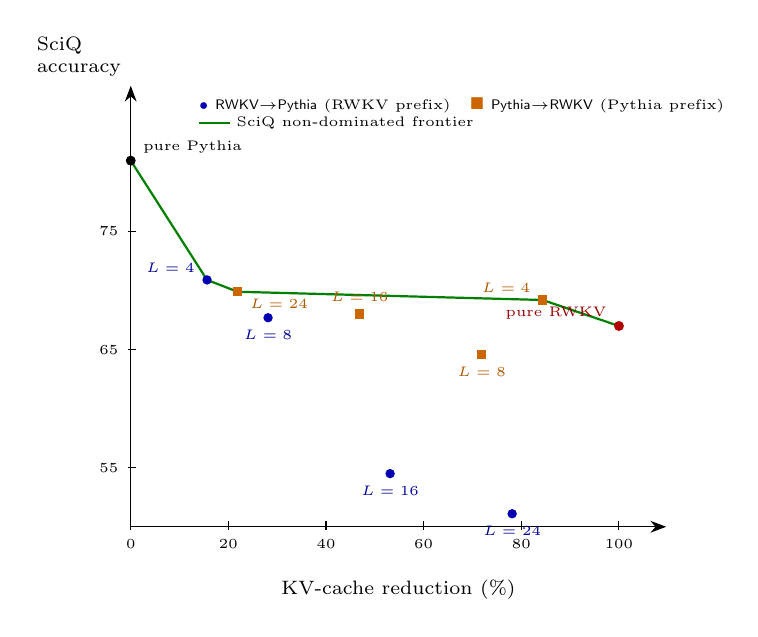
\begin{tikzpicture}[font=\scriptsize,>={Stealth[length=2mm]}]
  \def\xs{0.62}
  \def\ys{0.15}
  \draw[->] (0,0) -- (68mm,0);
  \draw[->] (0,0) -- (0,5.6) node[above left,font=\scriptsize,align=left] {SciQ\\accuracy};
  \node[font=\scriptsize] at (34mm,-8mm) {KV-cache reduction (\%)};
  \foreach \x in {0,20,40,60,80,100} \draw (\x*\xs/10,-1pt) node[below,font=\tiny]{\x} -- (\x*\xs/10,2pt);
  \foreach \y in {55,65,75} \draw (-1pt,{(\y-50)*\ys}) node[left,font=\tiny]{\y} -- (2pt,{(\y-50)*\ys});
  \coordinate (pP) at (0,{(81.0-50)*\ys});
  \coordinate (ab4) at ({15.625*\xs/10},{(70.9-50)*\ys});
  \coordinate (ab8) at ({28.125*\xs/10},{(67.7-50)*\ys});
  \coordinate (ab16) at ({53.125*\xs/10},{(54.5-50)*\ys});
  \coordinate (ab24) at ({78.125*\xs/10},{(51.1-50)*\ys});
  \coordinate (ba4) at ({84.375*\xs/10},{(69.2-50)*\ys});
  \coordinate (ba8) at ({71.875*\xs/10},{(64.6-50)*\ys});
  \coordinate (ba16) at ({46.875*\xs/10},{(68.0-50)*\ys});
  \coordinate (ba24) at ({21.875*\xs/10},{(69.9-50)*\ys});
  \coordinate (rw) at ({100*\xs/10},{(67.0-50)*\ys});
  \draw[green!50!black,thick] (pP)--(ab4)--(ba24)--(ba4)--(rw);
  \fill[black] (pP) circle (1.8pt);
  \foreach \p in {ab4,ab8,ab16,ab24} \fill[blue!70!black] (\p) circle (1.7pt);
  \foreach \p in {ba4,ba8,ba16,ba24}
    \node[fill=orange!80!black,rectangle,minimum size=3.4pt,inner sep=0pt] at (\p) {};
  \fill[red!70!black] (rw) circle (1.8pt);
  \node[above right=-1pt and 1pt of pP,font=\tiny] {pure Pythia};
  \node[above left=-1pt and 1pt of ab4,font=\tiny,text=blue!60!black] {$L=4$};
  \node[below=1pt of ab8,font=\tiny,text=blue!60!black] {$L=8$};
  \node[below=1pt of ab16,font=\tiny,text=blue!60!black] {$L=16$};
  \node[below=1pt of ab24,font=\tiny,text=blue!60!black] {$L=24$};
  \node[above left=-1pt and 1pt of ba4,font=\tiny,text=orange!70!black] {$L=4$};
  \node[below=1pt of ba8,font=\tiny,text=orange!70!black] {$L=8$};
  \node[above=1pt of ba16,font=\tiny,text=orange!70!black] {$L=16$};
  \node[below right=-1pt and 1pt of ba24,font=\tiny,text=orange!70!black] {$L=24$};
  \node[above left=-1pt and 1pt of rw,font=\tiny,text=red!60!black] {pure RWKV};
  \node[align=left,font=\tiny,fill=white,rounded corners=1pt,inner sep=2pt] at (42mm,5.25)
    {\textcolor{blue!70!black}{$\bullet$} \RtoP{} (RWKV prefix)\quad
     \textcolor{orange!80!black}{$\blacksquare$} \PtoR{} (Pythia prefix)\\
     \textcolor{green!50!black}{\rule[0.3ex]{4mm}{0.8pt}} SciQ non-dominated frontier};
\end{tikzpicture}}
\caption{SciQ accuracy vs.\ measured KV reduction for \RtoP{}/\PtoR{}. The non-dominated points across both paths are
pure Pythia $\to$ \RtoPL{4} $\to$ \PtoRL{24} $\to$ \PtoRL{4} $\to$ pure RWKV (green).
This is a post-hoc frontier on the single task SciQ,
and does not imply path-general superiority or generalization to unseen tasks.}
\label{fig:tradeoff}
\end{figure}
Adding the Pythia-prefix path yields the high-reduction point \PtoRL{4}. This point does not appear with the RWKV-prefix path alone.
Meanwhile, pure RWKV still has zero KV,
and \PtoRL{4} does not significantly exceed RWKV either. The benefit is therefore the ability to create \emph{additional trade-off points} between the frozen parents,
not that the new configurations uniformly dominate the parents.

\paragraph{Equal-KV Transformer baselines and an inference implementation with unused blocks removed.}We measured comparisons against efficiency baselines on the Transformer-parent side.
For \RtoP{}, compared with a Pythia early exit holding the same $31{-}L$ Transformer blocks, the chimeras at @16/@24 are higher by
ARC $+11.2/+18.5$ and SciQ $+12.8/+18.7$ points, while @4 is tied. For \PtoR{}, against early exits with the same $L{+}1=5/9/17/25$
blocks, the chimera is ARC $+35.4/+27.6/+16.9/+2.1$ and SciQ
$+38.7/+31.6/+17.9/+0.5$ points. The first three boundaries are significant, and at 25 blocks it is a tie (ARC $p{=}0.069$,
SciQ $p{=}0.80$): when the Pythia prefix is very shallow, the RWKV suffix supplies real function.

A path that physically removes the unused blocks is also implemented for \RtoP{}/\PtoR{}. For \PtoR{}, the Pythia prefix, the RWKV suffix, and the full path joining the two are
each compared against the unpruned reference, with $\mathrm{rel}{=}0$ at all $4$ boundaries. Resident weights are \RtoP{} $13.93$--$14.55$\,GiB and
\PtoR{} $13.49$--$14.11$\,GiB (the default \PtoRL{4} is $14.11$\,GiB), roughly half of the full pair of parents at $27$\,GiB. However, the corresponding
Pythia early exits are even lighter, $2.64$--$10.14$\,GiB for \PtoR{}. Furthermore, the reference runtime is not an optimized serving engine:
it runs HF RWKV sequentially along the sequence, and cacheless decode recomputes the prefix every time. \PtoRL{4} prefill at context $2048$ takes
$22.6$ seconds even after pruning (pure Pythia $0.378$ seconds), and unpruned cacheless decode runs at $0.148$ token/s
(Pythia $9.49$ token/s). These are figures of the current correctness-first implementation, not architecture-inherent speed limits.
Comparisons against KV quantization and sliding-window are also not performed.

The comparison against the parents comes with qualifications: \kw{function is preserved, but this is not a uniform improvement in accuracy}. Both \RtoP{} and \PtoR{}
fall significantly below the strong Pythia. \RtoP{} exceeds RWKV only on SciQ, and \PtoR{} does not significantly exceed RWKV at any boundary. The main benefit obtained is that
\PtoRL{4} removes $84.4\%$ of the Transformer KV while retaining part of Pythia's accuracy.

\paragraph{Translation is domain-specific.}The accuracies above were measured on short questions close to instruction format. KV-cache
savings matter for long contexts, and how well the chimera preserves \emph{open-text language modeling} there must be measured
separately. At context $512$, \RtoPL{4} has perplexity $6.40$ on Alpaca and $93.87$ on WikiText-103. \PtoRL{4} improves in both domains at
$3.85/45.00$, but WikiText still remains far from the parents' $11.33/16.22$. Extending the context to $2048$,
\PtoRL{4} reaches Alpaca $3.50$ and WikiText $34.78$, improving rather than collapsing. The main cause is therefore not context length but
\emph{domain shift}. \PtoR{} mitigates the shift, but WikiText $34.78$ is $4.2$ times the better parent RWKV's $8.27$,
and does not resolve the problem.

The linear control at each switch layer is a supervised affine oracle \emph{re-estimated separately} on the first $40{,}000$ tokens of Alpaca and of WikiText and
evaluated on the respective non-overlapping suffix. The WikiText values are not out-of-domain generalization of a mapping estimated on Alpaca, and they also differ from the trained
adapter in objective and data. Hence we do not conclude from the adapter-vs-affine comparison that ``only the nonlinear part overfit the domain.''
The evidence for domain specificity is that the same trained adapter changes its performance relative to the parents substantially between Alpaca and WikiText.

\begin{figure}[!htbp]\centering
\resizebox{\columnwidth}{!}{%
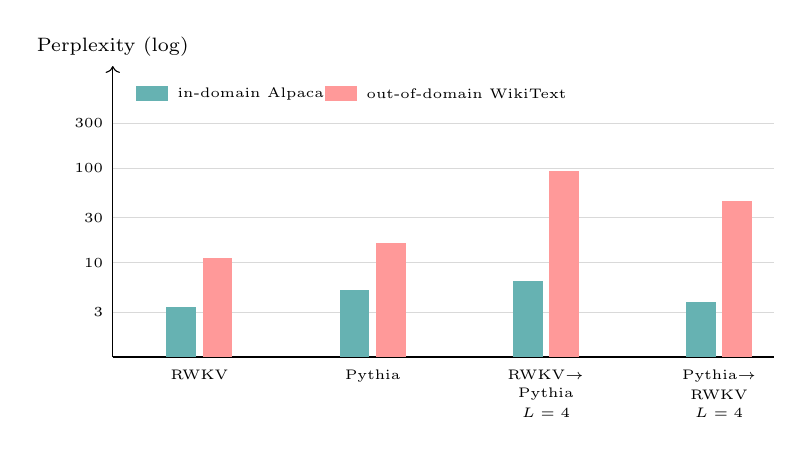
\begin{tikzpicture}[font=\scriptsize]
  % log-scale perplexity bars, in-domain (Alpaca) vs out-of-domain (WikiText), ctx 512. 1 decade = 1.2cm.
  \def\Y#1{ {12*ln(#1)/ln(10)/10} }
  \draw[->] (0,0) -- (0,3.7) node[above,font=\scriptsize] {Perplexity (log)};
  \foreach \v in {3,10,30,100,300} \draw[gray!30] (0,\Y{\v}) node[left,font=\tiny,black]{\v} -- (84mm,\Y{\v});
  \draw[thick] (0,0) -- (84mm,0);   % x baseline
  \def\grp#1#2#3#4{  % xcenter(mm), label, alpaca_ppl, wiki_ppl
    \fill[teal!60] (#1mm-4.2mm,0) rectangle (#1mm-0.4mm,\Y{#3});
    \fill[red!40]  (#1mm+0.4mm,0) rectangle (#1mm+4.2mm,\Y{#4});
    \node[font=\tiny,below=1pt] at (#1mm,0) {#2};
  }
  \grp{11}{RWKV}{3.42}{11.33}
  \grp{33}{Pythia}{5.19}{16.22}
  \grp{55}{\shortstack{RWKV$\to$\\Pythia\\$L=4$}}{6.40}{93.87}
  \grp{77}{\shortstack{Pythia$\to$\\RWKV\\$L=4$}}{3.85}{45.00}
  % legend in the empty top-left (above the short parent bars)
  \fill[teal!60] (3mm,3.25) rectangle (7mm,3.45);
  \node[font=\tiny,anchor=west] at (7mm,3.35) {in-domain Alpaca};
  \fill[red!40]  (27mm,3.25) rectangle (31mm,3.45);
  \node[font=\tiny,anchor=west] at (31mm,3.35) {out-of-domain WikiText};
\end{tikzpicture}}
\caption{Domain shift (context $512$, log axis). \PtoR{} improves the
WikiText perplexity of \RtoPL{4} from $93.87\to45.00$ but does not reach the parents' $11.33/16.22$. Because the same adapter
sits near the parents on Alpaca, domain, not length, is the primary difference.}
\label{fig:domain}
\end{figure}

\section{Related Work}\label{sec:related}
\paragraph{Model stitching.} Connecting the layers of $2$ frozen models through a trainable stitching layer was introduced by
Lenc and Vedaldi~\cite{10.1007/s11263-018-1098-y} to measure the \emph{equivalence} of representations, and was revisited by Bansal et al.~\cite{3540261.3540279} as a probe for representation comparison.
Both stitch within the \emph{same architecture and the same task}; our work differs in that it stitches different \emph{families} (RNN$\leftrightarrow$Transformer)
through a shared latent that translates each layer only $1$ time.
\paragraph{Composing frozen LLMs.} Recent work continues to compose frozen LLMs through trainable connections.
StitchLLM~\cite{hu-etal-2025-stitchllm} stitches blocks of Transformers of different scales with stitching layers and selects a
path at serving time, and BTS~\cite{zhang-etal-2025-bts} re-merges a set of experts branched from the same seed back into the seed with stitch layers.
CALM~\cite{bansal2024llm} fuses the intermediate representations of 2 frozen Transformers via cross-attention, and
Manticore~\cite{roberts2025pretrained} \emph{fine-tunes end-to-end} a hybrid that joins Transformer and Mamba blocks
with projections.
However, these either have Transformers on both sides (BTS uses a single seed) or fine-tune the composed model (Manticore). To our knowledge, no prior work translates the residuals of a frozen pure RNN and a frozen Transformer \emph{bidirectionally},
composes them at a single boundary, and goes as far as reporting the measured KV reduction.
\paragraph{Representation similarity.} CKA~\cite{pmlr-v97-kornblith19a} and (SV/PW)CCA~\cite{3295222.3295356,3327345.3327475} are standard tools for measuring representational
similarity between networks. Our work uses them as auxiliary metrics (the all-layer correspondence in \S\ref{sec:space}) while placing its main focus on
\emph{functional, reconstruction-mediated} stitching.
\paragraph{Model merging and knowledge fusion.} Methods that merge models in weight space---model soups~\cite{pmlr-v162-wortsman22a}, TIES~\cite{3666122.3666432}, and evolutionary merging~\cite{Akiba2025}---
presuppose \emph{identical or compatible} weights. FuseLLM~\cite{wan2024knowledge}, which fuses output distributions, does not require weight compatibility,
but it needs token alignment across vocabularies and continued training of the target model. Our work is complementary in that it merges
no weights at all and instead translates the \emph{activation space} to recombine frozen blocks.
\paragraph{Target models.} RWKV~\cite{peng-etal-2023-rwkv} is an architecture that has no softmax self-attention and operates as a pure recurrence at inference time; Pythia~\cite{3618408.3618510} and its Tulu SFT
variant are Transformers. The fact that the two share the GPT-NeoX tokenizer is what makes position-aligned residual pairs possible.

\section{Discussion}\label{sec:discussion}
In our experiments, a shared representation can be learned between corresponding layers of frozen heterogeneous families ($\rho_{\mathrm{ctr}}\!=\!0.90$).
\kw{However, the scope of this claim is limited}: the correspondence in this work is measured under the favorable conditions of
\emph{an identical tokenizer, identical width, identical layer count, identical inputs, and a domain close to Alpaca};
the shuffled control rules out token-independent distribution matching, but we do not disentangle whether the observed correspondence
stems from semantics, vocabulary, position, or syntax. Indeed, the substantial degradation of translation on out-of-domain WikiText (\S\ref{sec:goal}) indicates that this may be a
\emph{representation transformation specific to the training domain}. Hence it is more accurate to read this not as a ``general shared \emph{semantic} space'' but as a ``shared space of
token-aligned representations under favorable conditions.'' It is also important that high latent correlation does not guarantee high read-out accuracy; the presence of a shared representation and
decodability must be evaluated separately. A chimera built on this space functions, but at a loss, and in the generation samples both paths remain fluent
while erring in content or form. Moreover, the fact that \PtoR{} substantially outperforms \RtoP{} at deep boundaries shows that
local $R^2$ or layer index alone cannot predict end-to-end performance, and that which parent is placed as the prefix matters.
A competitive chimera requires identifying the factors that bottleneck $B\!\to\!B$
(including a $\sigma$ sweep), training across domains, and selecting complementary parent models on the pretraining side.

\paragraph{Limitations.} Adapter training uses only a single random seed. The evaluation texts were obtained by splitting the instruction data without overlap,
so by construction no training data can leak into them, and the gap between training-time and evaluation-time performance persisting to the end corroborates this; however, at the $7$B scale
we did not go as far as an $n$-gram audit. Performance is measured on the \kw{full evaluation sets} (ARC-Easy $2376$, SciQ $1000$), and differences between configurations
were assessed with paired tests on the same questions (McNemar's exact test and paired bootstrap). \RtoP{} exceeds the weaker parent only on SciQ, and only under the length-normalized score (it does not hold under the sum score), and
\PtoR{} does not significantly exceed RWKV at any boundary. We evaluate $2$ tasks $\times2$ cross paths $\times4$ switches plus multiple controls, without
correction for multiple comparisons. The two direction-fixed released runtimes both take $L{=}4$ as the default, but this was
post-hoc selected from the four boundaries of each path on the same two test sets, with no independent selection/confirmation split.
The identical-adapter intervention on the nonlinear branch was performed at the same layers and questions for both \RtoP{}/\PtoR{}, but it is an intervention on a single checkpoint
and may not generalize to different adapter training conditions.
Moreover, the composition always has only a single boundary, and we did not measure how translation error accumulates across multiple boundaries. Furthermore, the chimera evaluation is
likelihood-based, which measures the ability to \emph{select} the correct option and does not directly measure the ability to \emph{generate}.
The four generation samples each for \RtoP{}/\PtoR{} are only a qualitative supplement, not a comprehensive evaluation of generation ability. In addition, the translation is
\emph{specialized to the training domain} and degrades substantially on WikiText. Long-context CE is measured at contexts $512$/$1024$/$2048$ (capped at $2048$ because both parents
are models with context length $\le 2048$). This is language-modeling quality and does not directly measure reading comprehension requiring long-range
dependencies. Regarding the inference implementation, we measured that actually removing the unused blocks reduces the resident weights by about half
(\S\ref{sec:goal}); however, the correctness-first unpruned runtime recomputes the prefix cachelessly, and HF RWKV also runs sequentially, so
the chimera is about $63$--$70\times$ slower than pure Pythia in prefill/decode. This is an implementation property, not a property of the architecture, and
latency and throughput on an optimized inference path are left for future work. We also did not perform an equal-memory comparison against KV quantization or sliding-window approaches. Ablations over $\sigma$, $\lambda$, latent width, the number of residual blocks, and
the amount of training data, as well as alignment on a same-family pair (identical architecture), were not conducted in this $32$-layer configuration and
are left for future work.

{\small
\bibliographystyle{IEEEtran}
\bibliography{reference}}

\appendices

\section{Reproduction Information}\label{sec:repro}
\begin{itemize}\setlength{\itemsep}{1pt}
\item \kw{Models}: RWKV-Raven-7B (BlinkDL \texttt{.pth} converted to HF format and re-saved in fp16) and
\texttt{allenai/open-instruct-pythia-6.9b-tulu} (fp16). Both have $32$ layers, $d{=}4096$, and the GPT-NeoX-20B tokenizer.
\item \kw{Adapter}: $z{=}d{=}4096$, $1$ residual block (inner width $4096$, second matrix zero-initialized), non-affine LN,
$\sigma{=}0.4$, $\lambda{=}1$, $268.5$M parameters. AdamW, effective batch $4096$ on $4{\times}$V100, learning rate $10^{-3}\!\to\!10^{-5}$
($\times0.5$ whenever held-out $A\!\to\!B$ stops improving), a $416{,}000$-iteration run (the reported checkpoint is the one at $415{,}000$ iterations, best on held-out $A\!\to\!B$), random seed $0$.
\item \kw{Data}: residuals are taken from the leading portion of the Alpaca training split (windows of $112$ tokens, $\approx\!232$k independent token positions), and evaluation windows are taken from
character position $2{,}000{,}000$ onward (a fixed offset independent of $N$); the two do not overlap. Standardization statistics are computed from each layer's training residuals
and used for de-standardization.
\item \kw{Evaluation}: held-out $\Rsq$ is computed at each layer by pooling all tokens and all dimensions (SST is centered per dimension; exact metric definitions are given in Appendix~\ref{sec:common-mode}), and we report the simple mean over the $32$ layers. Multiple choice is decided by the
log-likelihood of the sequence formed by concatenating each option (sum/mean over the tokens after the prompt), using the full evaluation sets (ARC-Easy test $2376$, SciQ test $1000$).
SciQ is evaluated in closed-book form without the support passage.
Differences between configurations are assessed with paired tests (McNemar and paired bootstrap). For the RWKV suffix of \PtoR{}, options are always evaluated at batch $1$;
concatenating controls along the batch axis produced per-layer differences of $\mathrm{rel}{=}8.3{\times}10^{-4}$--$1.8{\times}10^{-3}$ and was therefore rejected, and only the path that keeps batch $1$ while
parallelizing over independent CUDA streams is used, after passing a $\mathrm{rel}<10^{-4}$ gate against sequential execution.
\PtoR{} is likewise fixed to the same distributed checkpoint as \RtoP{}, step $415{,}000$ selected on held-out $A\!\to\!B$;
no re-selection of checkpoints that saw $B\!\to\!A$ or \PtoR{} QA is performed. However, the two direction-fixed released runtimes
take as default the $L{=}4$ whose reported test mean was highest over the four boundaries of each path after evaluation, with no independent deployment-selection split.
\item \kw{Code and structured data}: the repository for this work is
\href{https://github.com/kotama7/NinaXander}{\texttt{https://github.com/kotama7/NinaXander}}
(a private repository as of July 30, 2026; publication planned). It contains the experiment code, the raw data of each evaluation together with
aggregate tables of the values reported in the paper, the reproduction procedure, and checks that automatically cross-verify the numbers in the text against the tabulated data.
Details of the hook-capture consistency checks, boundary gates, training runs and convergence records, noise-ceiling analysis, and the fitting procedure for the affine control
are documented in the repository documentation (\texttt{docs/}).
\item \kw{Hugging Face distributions}: the inference artifacts as of July 30, 2026 were stored in the following three private model
repositories. Access requires the owner's approval, and they are not visible to unauthenticated readers.
The private collection grouping the three is
\hfcollection
  {https://huggingface.co/collections/kotama7/ninaxander-private-inference-releases-6a6b02ec40c18d6b41ed040a}
  {ninaxander-private-inference-releases-6a6b02ec40c18d6b41ed040a}.
\begin{itemize}\setlength{\itemsep}{0pt}
\item Shared adapter: \hfrepo
  {https://huggingface.co/kotama7/ninaxander-raven7b-tulu69-adapter}
  {ninaxander-raven7b-tulu69-adapter}
\item \PtoR{} (default $L{=}4$): \hfrepo
  {https://huggingface.co/kotama7/ninaxander-tulu69-to-raven7b-best}
  {ninaxander-tulu69-to-raven7b-best}
\item \RtoP{} (default $L{=}4$): \hfrepo
  {https://huggingface.co/kotama7/ninaxander-raven7b-to-tulu69-best}
  {ninaxander-raven7b-to-tulu69-best}
\end{itemize}
Each repository includes model cards and notices in English, Japanese, and Simplified Chinese, SafeTensors, and a SHA-256 manifest.
All distribution licenses follow the more restrictive parent (Tulu-Pythia), namely the AI2 AI Model License (non-commercial research only),
and each NOTICE records attribution to the parent models.
\end{itemize}

\section{Metric Definitions and Detailed Common-Mode Analysis}\label{sec:common-mode}
This section gives rigorous definitions of the metrics and supplementary material on the common-mode correction of \S\ref{sec:space}--\S\ref{sec:ladder}.

\paragraph{Metric definitions.}Residuals are standardized per layer using the per-dimension means and standard deviations estimated from the training tokens
(and de-standardized at chimera insertion). All three loss terms are means over all elements (tokens ${\times}$ dimensions), and
since $z$ has unit variance under the non-affine LN, $\lambda{=}1$ amounts to adding the per-element errors on the same scale.
The noise $\xi_A,\xi_B$ is sampled independently for each branch.
$\Rsq$ is computed per layer as
$1-\mathrm{SSE}/\mathrm{SST}$, pooling the held-out tokens and all $4096$ dimensions. SST is the total variation after removing the per-dimension token mean, so dimensions with larger variance
contribute more. There are two held-out sets: the training-time evaluation that provides the headline values and the learning curves uses $1{,}000$ windows ${\times}\,112=112{,}000$ tokens, while the per-layer analysis and the shuffle control (\S\ref{sec:space}) use $400$ windows ${\times}\,112=44{,}800$ tokens; because the evaluation sets differ, the $32$-layer averages in the per-layer table ($0.561/0.592$) do not exactly match the headline values ($0.559/0.590$). $\rho_{\mathrm{ctr}}$ is a single Pearson correlation computed after removing each dimension's token mean within a layer and then
flattening (tokens ${\times}$ dimensions). In $f=\lVert z-\overline z\rVert^2/\lVert z\rVert^2$, $\overline z$ is
the per-dimension token mean within a layer, computed for each of models $A$ and $B$ and averaged. Every metric is computed per layer, and we report the
simple average over the $32$ layers. The fit $R^2$ over all layer correspondences in \S\ref{sec:space} is an in-sample ridge linear probe, fit and evaluated on the same $22{,}400$ rows for each layer pair.

\paragraph{What $f$ does and does not show.}$f$ is a second moment, not a measure of information, and the inferences it licenses run in one direction
only. $f\!\to\!0$ proves that the latent has collapsed to a constant, and hence that it carries no per-token information at all
--- detecting this degeneracy is precisely why $f$ was introduced. The converse does not hold, and indeed this appears in the training process of this very study.
At iteration $0$, after a single update from random initialization, $f{=}0.926$ --- the
maximum over the entire training run --- yet all four read-outs at that same point are negative (in the order \RWKVself{}/\RtoP{}/\Pythiaself{}/\PtoR{},
$-0.042/-0.108/-0.029/-0.135$) --- that is, worse than predicting the token mean.
A large $f$ means only that the per-token latents are spread out in angular direction;
under layer normalization without elementwise gains, $f$ is strictly invariant to scaling. Spread arises equally from meaningful variation and from meaningless
variation. Consequently, it is the read-out, not $f$, that can claim ``the varying component carries information''; and since the read-out is a
\kw{centered $R^2$}, any token-independent predictor scores exactly $0$. $B\!\to\!B=0.711$ cannot be obtained from any
constant. Moreover, the two must be read together. In the latter half of training ($85{,}000\!\to\!415{,}000$ iterations), while $f$ increases $0.189\!\to\!0.350$,
$\rho_{\mathrm{ctr}}$ \emph{falls} $0.949\!\to\!0.901$, because part of the added spread is variation on which the two families
do not agree.

\paragraph{Raw correlation fails to capture improvement: an example from the training dynamics.}Over iterations $58{,}000\!\to\!66{,}000$, after the learning rate has dropped, $f$ increases
$0.138\!\to\!0.153$, and $\rho_{\mathrm{ctr}}$ ($0.950\!\to\!0.952$) and the four read-outs
(\RWKVself{} $0.562\!\to\!0.570$, \RtoP{} $0.477\!\to\!0.486$, \Pythiaself{} $0.545\!\to\!0.552$,
\PtoR{} $0.504\!\to\!0.514$) all improve together. Yet over the same interval $\rho_{\mathrm{raw}}$ goes from $0.9931$ to
$0.9927$ --- if anything, a slight \emph{decrease}. Even as the model replaces the common mode with token-dependent information that can be read out, the raw correlation captures
none of the improvement. This exemplifies exactly why alignment quality must not be measured with raw correlation.

\paragraph{Trajectory of $f$ in the wide latent.}Because nearly all of the latent's energy can fit into the common mode,
the wide latent collapses early in training to $f\!\approx\!0.02$ --- $98\%$ of the latent being a token-independent constant ---
($f{=}0.015$ at $1{,}000$ iterations). Recovery from there is slow: even at $25{,}000$ iterations $f$ is only $0.058$, and at $85{,}000$
iterations still $0.189$; the deepest point of recovery, $0.350$, is reached only in the final stage of training. Even at that value,
\kw{$65\%$ of the latent's energy is a shared constant}, and only the remaining $35\%$ \emph{can} carry
per-token information.

\balance
\end{document}
